\section{Data Extraction \& Analysis}

A web crawler will be created using python that will enable website content to be extracted. The Python library that will be used is Scrapy which will handle visiting of the websites when provided a list of hosts. Scrapy will then crawl through all directories within the host (defined by the websites robot.txt). After visiting a URL, the content will be extracted and analysed using information retrieval methods through the use of the Python Natural Language Toolkit (NLTK) library. Below shows a flow diagram for the information retrieval process.

\begin{figure}
  \centering
  \begin{minipage}{7cm}
    \centering
    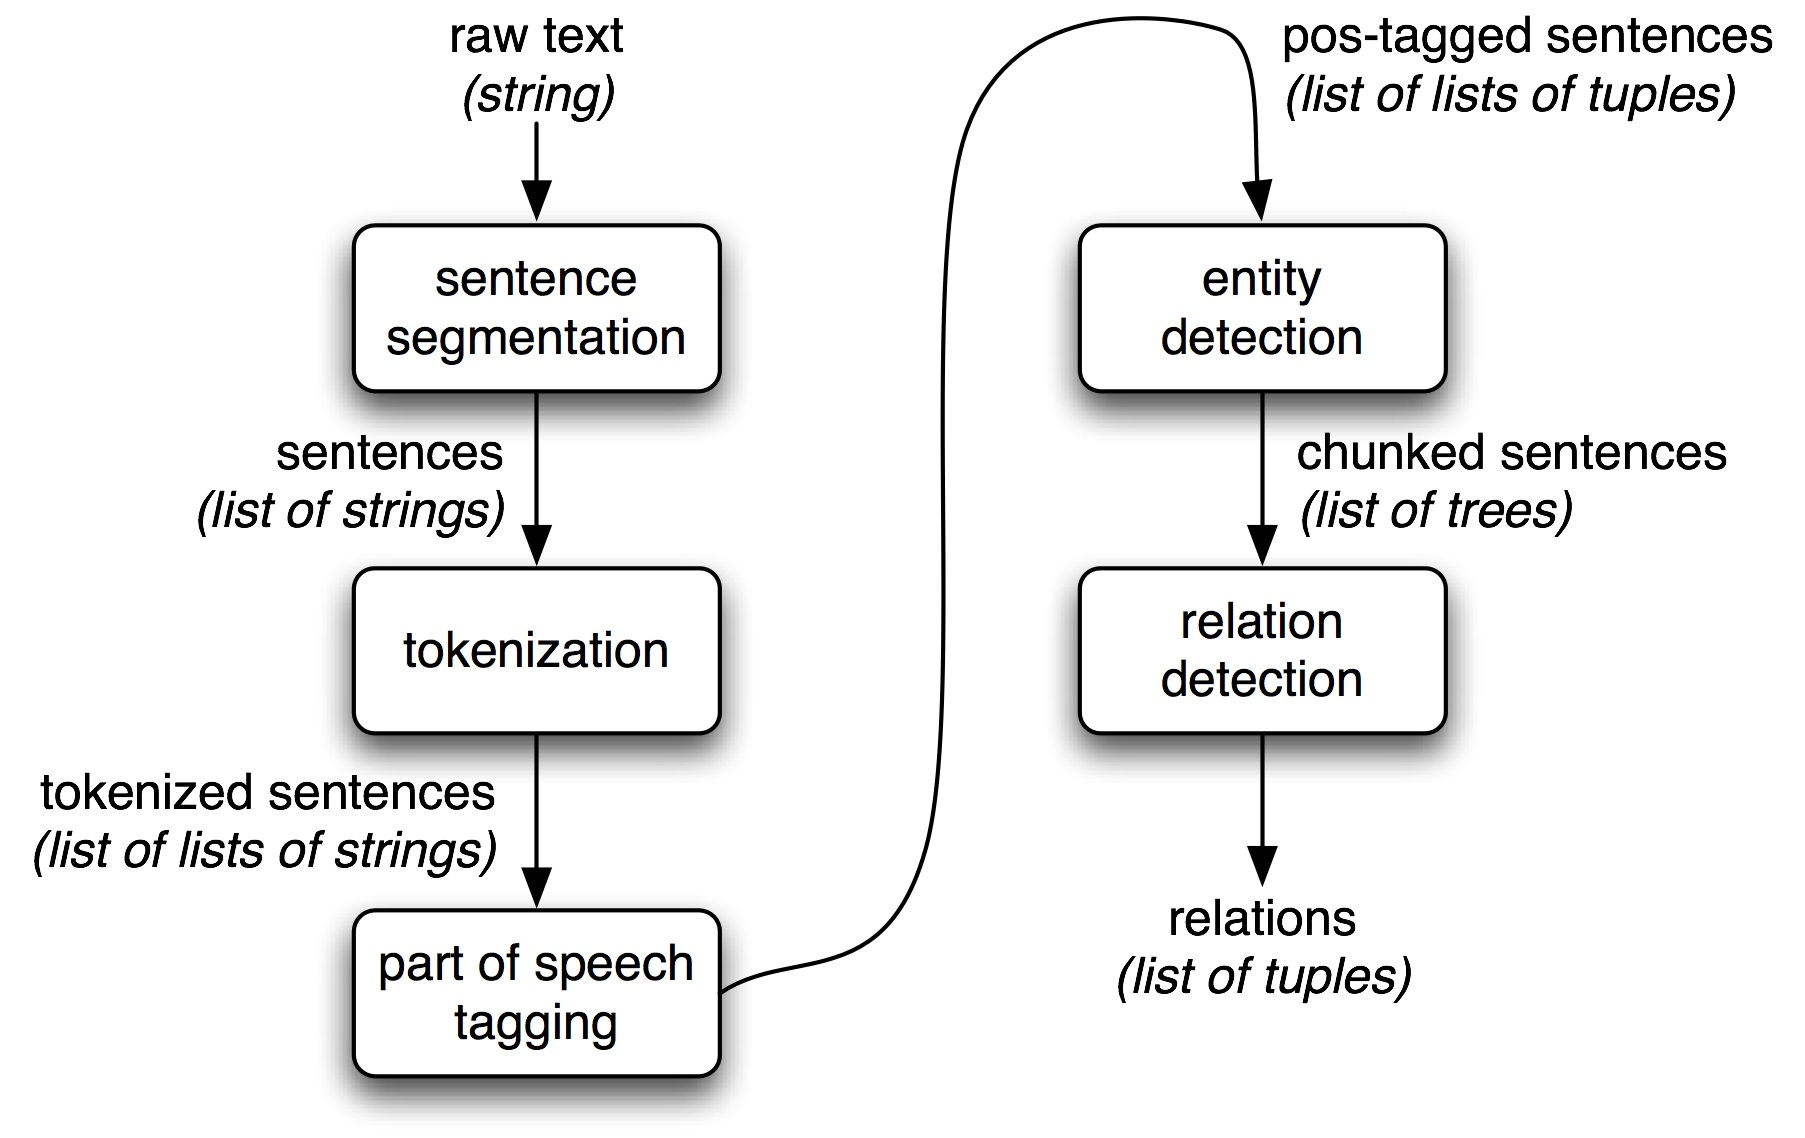
\includegraphics[width=7cm]{inc/ie-architecture.jpg}
    \caption{Python Natural Language Tookit Information retrieval flow diagram}
    \label{fig:information_retrieval}
  \end{minipage}
\end{figure}

Many websites implement measures to prevent web crawlers from crawling due to the number of requests made, eating up at their resources. Usually this results in the web crawling server being banned. However, there are measures to prevent this explained below.

\begin{itemize}
  \item Disabling cookies may prevent getting banned if it’s the method used by the website to detect crawlers.
  \item Using Google cached pages instead of visiting the websites directly.
  \item Use different IPs by rotating from a list when making a request to the same host.
  \item Setting a delay between requests.
\end{itemize}
